\section{Verifica al ribaltamento (GEO, A1 M1 R3)}
Il ribaltamento della struttura è il fenomeno che si genera quando, considerando il punto (fulcro) R, il momento stabilizzante è inferiore rispetto al momento destabilizzante.
\begin{figure}[H]
    \centering
    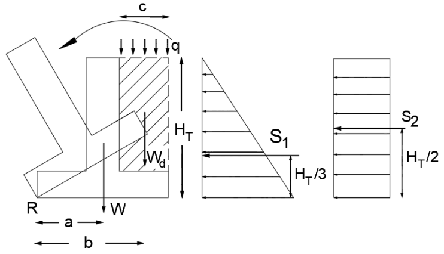
\includegraphics[width=0.5\textwidth]{immagini/ribaltamento.png} \hfill
        \caption{Schematizzazione del fenomeno di ribaltamento che interessa il muro.}
    \label{figure:pesi_muro}
\end{figure}
Secondo la NTC-2018, la verifica al ribaltamento è accettata nel caso in cui la resistenza di progetto ($R_d$) è maggiore o uguale rispetto all'azione di progetto ($E_d$).\\
La resistenza di progetto è pari al prodotto tra i momenti stabilizzanti ed un coefficiente di riduzione, mentre l'azione di progetto è il prodotto tra un coefficiente di sicurezza ed i momenti destabilizzanti:
\begin{equation*}
    \gamma_{G1_{Rd}} \cdot \frac{M_{STAB}}{\gamma_R} \geq \gamma_{G1_{Ed}} \cdot M_{DESTAB}
\end{equation*}
Dove:
\begin{itemize}
    \item $\gamma_{G1_{Rd}}$ = 1.00;
    \item $\gamma_R$ = 1.15;
    \item $\gamma_{G1_{Ed}}$ = 1.30.
\end{itemize}
%\subsection{Momenti stabilizzanti}
\textbf{Muro}
\begin{equation*}
    M_1 = W_1 \cdot \left(a + \frac{s}{2}\right) = 37500 \cdot \left(0.4 + \frac{0.5}{2}\right) = 24375 \,N m
\end{equation*}
\textbf{Fondazione}
\begin{equation*}
    M_2 = W_2 \cdot \frac{B}{2} = 33125 \cdot \frac{2.65}{2} = 43890 \, Nm
\end{equation*}
\textbf{Terreno}
\begin{equation*}
    M_3 = W_3 \cdot \left(a + s + \frac{t}{2}\right) = 97650 \cdot \left(0.4 + 0.5 + \frac{1.75}{2}\right) = 173328 \,Nm
\end{equation*}
\textbf{Carico permanente}
\begin{equation*}
    M_q = W_q \cdot \left(a + s + \frac{t}{2}\right) = 10500 \cdot \left(0.4 + 0.5 + \frac{1.75}{2}\right) = 18637 \,Nm
\end{equation*}
\textbf{Momento stabilizzante}
\begin{equation*}
    M_{STAB} = M_1 + M_2 + M_3 + M_q = 24375 + 43890 + 173328 + 18637 = 260231 \,Nm
\end{equation*}

%\subsection{Momenti destabilizzanti}
\textbf{Spinta attiva}
\begin{equation*}
    M_{S1} = S_1 \cdot \frac{1}{3} H_t = 37975 \cdot \frac{1}{3} \cdot 3.5 = 44304\, Nm
\end{equation*}
\textbf{Spinta del carico permanente}
\begin{equation*}
    M_{Sq} = S_q \cdot \frac{1}{2} H_t = 7000 \cdot \frac{1}{2} \cdot 3.5 = 12250 \,Nm
\end{equation*}
\textbf{Momento destabilizzante}
\begin{equation*}
    M_{DESTAB} = M_{S1} + M_{Sq} = 44304 + 12250 = 56554 \,Nm
\end{equation*}

\textbf{Resistenza di progetto}
\begin{equation*}
    R_d = \frac{\gamma_{G1 \cdot M_{STAB}}}{\gamma_R} = \frac{1 \cdot 260231}{1.15} = 226289 \,Nm
\end{equation*}
\textbf{Azione di progetto}
\begin{equation*}
    E_d = \gamma_{G1} \cdot M_{DESTAB} = 1.3 \cdot 56554 = 73520 \,Nm
\end{equation*}
Essendo che la resistenza è superiore all'azione di progetto, la verifica a ribaltamento del muro è accettata.

\section{Verifica a scorrimento (GEO, A1 M1 R3)}
Il fenomeno dello scorrimento avviene nel caso in cui la componente orizzontale totale delle spinte è superiore rispetto all'attrito che si genera tra la fondazione del muro ed il terreno sottostante.
\begin{figure}[H]
    \centering
    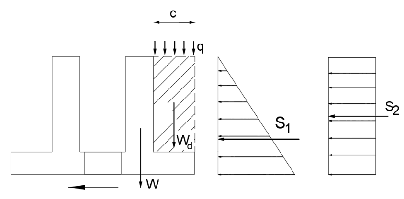
\includegraphics[width=0.5\textwidth]{immagini/scorrimento.png} \hfill
        \caption{Schematizzazione del fenomeno di scorrimento che interessa il muro.}
    \label{figure:pesi_muro}
\end{figure}
Secondo le NTC-2018, la verifica a scorrimento necessita che vengano presi in considerazione la resistenza e l'azione di progetto, ovvero le forze stabilizzanti ed instabilizzanti moltiplicate per certi coefficienti. La verifica viene accettata se la resistenda $R_d$ è superiore rispetto all'azione $E_d$.
\begin{equation*}
    \gamma_{G1} = \frac{F_{STAB} \cdot tan(\delta)}{\gamma_R} \geq \gamma_{G1} \cdot F_{DESTAB}
\end{equation*}
Dove: 
\begin{itemize}
    \item $\gamma_{G1_{Rd}} = 1.00$;
    \item $\gamma_R$ = 1.10;
    \item $\gamma_{G1_{Ed}} = 1.30$
\end{itemize}
\textbf{Resistenza di progetto}
\begin{equation*}
    R_d = \gamma_{G1} \cdot \frac{F_{STAB} \cdot tan(\delta)}{\gamma_R} = 1.00 \cdot \frac{178775 \cdot tan(33)}{1.10} = 59153 \,N
\end{equation*}
Dove:
\begin{equation*}
\delta = \frac{2}{3}  \cdot \phi = \frac{2}{3} \cdot 30° = 20°
\end{equation*}
\textbf{Azione di progetto}
\begin{equation*}
    E_d = \gamma_{G1} \cdot F_{DESTAB} = 1.3 \cdot 44975 = 58468 \,N
\end{equation*}
Essendo che la resistenza di progetto è superiore rispetto all'azione di progetto, la verifica allo scorrimento del muro è accettata.

\section{Verifica della capacità portante terreno-fondazione (GEO, A1 M1 R3)}
Mediante questa verifica si procede a valutare se il terreno sotto la fondazione dell'opera è in grado di sostenere il peso del muro stesso e del volume di terreno sopra il tacco.\\
Questo accertamento permette di prevedere la possibilità che si verifichi un cedimento del terreno, e di conseguenza un collasso del muro.\\
Anche per questa verifica, la resistenza di progetto dev'essere almeno uguale all'azione di progetto.
\begin{equation*}
    \gamma_{G1} \cdot \frac{Q_{lim}}{\gamma_R} \geq \gamma_{G1} \cdot F_{STAB}
\end{equation*}
Dove: 
\begin{itemize}
    \item $\gamma_{G1_{Rd}} = 1.00$;
    \item $\gamma_R$ = 1.40;
    \item $\gamma_{G1_{Ed}} = 1.00$ 
\end{itemize}
\textbf{Base reagente}
\begin{equation*}
    B_r = 2 \cdot \frac{\gamma_{G1} \cdot M_{STAB} - \gamma_{G1} \cdot M_{DESTAB}}{\gamma_{G1} \cdot F_{STAB}} = 2 \cdot \frac{1 \cdot 26231 - 1.3 \cdot 56554}{1 \cdot 178775} = 2.09 \,m
\end{equation*}

\textbf{Capacità portante}
\begin{equation*}
\begin{split}
    q_{lim} = \frac{1}{2} \cdot (\gamma_D \cdot B_r \cdot N_{\gamma} \cdot S_{\gamma} \cdot i_{\gamma} \cdot g_{\gamma}) + (\gamma_D \cdot D \cdot N_q \cdot S_q \cdot d_q \cdot i_q) =\\
    0.5 \cdot (18600 \cdot 2.09 \cdot 20.09 \cdot 1.06 \cdot 0.326) + (18600 \cdot 0.5 \cdot 18.40 \cdot 1.06 \cdot 1.12 \cdot 0.326) =\\
     255516 \,N/m^2
\end{split}
\end{equation*}
\textbf{Fattori di capacità portante}
\begin{equation*}
    N_q = e^{\pi \cdot tan(\phi)} \cdot tan^2 \left(45 + \frac{\phi}{2}\right) = e^{\pi \cdot tan(30)} \cdot tan^2 \left(45 + \frac{30}{2}\right) = 18.40 
\end{equation*}
\begin{equation*}
    N_{\gamma} = 2 \cdot (N_q -1) \cdot tan(\phi) = 2 \cdot (18.40 -1) tan (30) = 20.09
\end{equation*}
\textbf{Fattori di forma}
\begin{equation*}
    S_{\gamma} = S_q = 1+0.1 \cdot \left(\frac{B_r}{LL}\right) \cdot \frac{1+sen(\phi)}{1-sen(\phi)} = 1 + 0.1 \cdot \left(\frac{2.09}{10}\right) \cdot \frac{1+sen(30)}{1-sen(30)} = 1.06
\end{equation*}
\textbf{Fattori di inclinazione del carico}
\begin{equation*}
    i_{\gamma} = i_q = \left(1- \frac{\gamma_{G1} \cdot F_{DESTAB}}{\gamma_{G1} \cdot F_{STAB} + B_r \cdot LL}\right) ^{m+1} = \left(1- \frac{1.3 \cdot 44975}{1 \cdot 178775 + 2.09 \cdot 10}\right) ^{1.83+1} = 0.326
\end{equation*}
\begin{equation*}
    m= \frac{2+ \frac{B_r}{LL}}{1+ \frac{B_r}{LL}} = \frac{2+ \frac{2.09}{10}}{1+ \frac{2.09}{10}} = 1.83
\end{equation*}
\textbf{Fattore di profondità}
\begin{equation*}
    d_q = 1+ 2 \cdot tan(\phi) \cdot (1- sen(\phi))^2 \cdot \frac{D}{B_r} = 1+ 2 \cdot tan(30) \cdot (1- sen(30))^2 \cdot \frac{0.9}{2.09} = 1.12
\end{equation*}
\begin{equation*}
    D = h_f + D_p = 0.5 + 0.4 = 0.9 \,m
\end{equation*}
\textbf{Carico limite del terreno}
\begin{equation*}
    Q_{lim} = q_{lim} \cdot B_r \cdot 1 = 255516 \cdot 2.09 = 533720 \,N
\end{equation*}

\textbf{Resistenza di progetto}
\begin{equation*}
    R_d = \gamma_{G1} \cdot \frac{Q_{lim}}{\gamma_r} = 1.00 \cdot \frac{533720}{1.40} = 381228 \,N
\end{equation*}
\textbf{Azione di progetto}
\begin{equation*}
    E_d = \gamma_{G1} \cdot F_{STAB} = 1.00 \cdot 178775 = 178775 \,N
\end{equation*}

Essendo che la resistenza di progetto è superiore rispetto all'azione, la capacità portante terreno-fondazione è verificata.

\section{Verifiche strutturali}
Le verifiche che riguardano la struttura del muro vengono svolte considerando tre porzioni dell'opera:
\begin{itemize}
    \item sezione 1: sezione orizzontale alla base del muro;
    \item sezione 2: sezione verticale della mensola di fondazione in corrispondenza dell'inizio del tacco;
    \item sezione 3: sezione verticale della mensola di fondazione in corrispondenza dell'inizio della punta.
\end{itemize}
Le forze che agiscono sul muro in modo orizzontale creano una sollecitazione di taglio. Il peso del muro genera invece una sollecitazione normale alla sezione orizzontale del muro, ovvero una pressoflessione. Le sezioni della fondazione (tacco e punta), sono soggette ad una sollecitazione di taglio e momento, entrambi distribuite in modo lineare.
\begin{figure}[H]
    \centering
    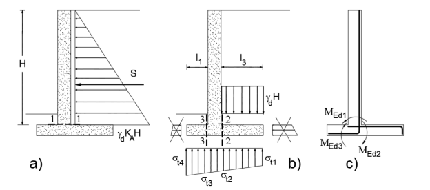
\includegraphics[width=0.7\textwidth]{immagini/stati_limiti_strutturali.png} \hfill
        \caption{Schematizzazione delle tensioni agenti sulle varie sezioni del muro.}
    \label{figure:stati_limit_strutturali}
\end{figure}

\subsection{Sezione 1}
La sezione 1 dell'opera interessa l'altezza del muro (escludendo la fondazione) e lo spessore del muro s.\\
Su questa sezione si valuta il momento flettente e lo sforzo di taglio, generati dal carico permanente q e dalla spinta attiva del terreno rispetto al punto C.\\
\textbf{Spinte rispetto a C}
\begin{equation*}
    S_{1C} = \frac{1}{2} \cdot \gamma_D \cdot K_a \cdot H^2 = \frac{1}{2} \cdot 18600 \cdot 0.33 \cdot 3^2 = 27900 \,N/m
\end{equation*}
\begin{equation*}
    S_{qC} = q \cdot K_a \cdot H = 6000 \cdot 0.33 \cdot 3 = 6000 \,N/m
\end{equation*}
\begin{equation*}
    F_{ORIZ} = S_{1C} + S_{qC} = 27900 + 6000 = 33900 \,N/m
\end{equation*}
\textbf{Momenti stabilizzanti rispetto a C}
\begin{equation*}
M_{S_{1C}} = S_{1C} \cdot \frac{H}{3} = 27900 \cdot \frac{3}{3} = 27900 \,Nm    
\end{equation*}
\begin{equation*}
M_{S_{qC}} = S_{qC} \cdot \frac{H}{2} = 6000 \cdot \frac{3}{2} = 9000 \,Nm    
\end{equation*}
\begin{equation*}
    M_{Stot} = M_{S_{1C}} + M_{S_{qC}} = 27900 + 9000 = 36900 \,Nm
\end{equation*}
\textbf{Momento destabilizzante rispetto a C}
\begin{equation*}
    M_{Ed1} = \gamma_{G1} \cdot M_{Stot} = 1.3 \cdot 36900 = 47970\, Nm
\end{equation*}
\textbf{Sforzo di taglio rispetto a C}
\begin{equation*}
    V_{Ed1} = \gamma_{G1} \cdot F_{ORIZ} = 1.3 \cdot 33900 = 44070 \,N
\end{equation*}

\subsection{Sezione 2 e 3}
Nelle sezioni 2 e 3 del muro si generano delle sollecitazioni di momento e di taglio. Inoltre, nella sezione 2 si generano delle ulteriori tensioni di momento e taglio dovute al peso del terreno che grava sul tacco.\\
\textbf{Sforzo normale}
\begin{equation*}
    N = F_{VERT} = 178775 \,N
\end{equation*}
\textbf{Momento}
\begin{equation*}
    M = N \cdot e_g = 178775 \cdot 0.28 = 50165 \,Nm
\end{equation*}
\textbf{Eccentricità}
\begin{equation*}
    e_c = \frac{B_r}{2} = \frac{2.09}{2} = 1.04 \,m
\end{equation*}
\begin{equation*}
    e_g = \frac{B}{2} - e_c = \frac{2.65}{2} - 1.04 = 0.28\, m
\end{equation*}
\textbf{Momento d'inerzia}
\begin{equation*}
    J = \frac{1}{12} \cdot B^3 = \frac{1}{12} \cdot 2.65^3 = 1.55 \,m^4
\end{equation*}
\textbf{Tensioni}
\begin{equation*}
    \sigma_{t1} = \frac{N}{B} - \left(\frac{M}{J} \cdot \frac{B}{2}\right) = \frac{178775}{2.65} - \left(\frac{50165}{1.55} \cdot \frac{2.65}{2}\right) = 24601 \, N/m^2
\end{equation*}
\begin{equation*}
    \sigma_{t2} = \frac{N}{B} - \left(\frac{M}{J} \cdot \left(\frac{B}{2} -t\right)\right) = \frac{178775}{2.65} - \left(\frac{50165}{1.55} \cdot \left(\frac{2.65}{2} -1.75\right)\right) = 81210 \,N/m^2
\end{equation*}
\begin{equation*}
    \sigma_{t3} = \frac{N}{B} + \left(\frac{M}{J} \cdot \left(s + t - \frac{B}{2}\right)\right) = \frac{178775}{2.65} + \left(\frac{50165}{1.55} \cdot \left( 0.5+1.75 - \frac{2.65}{2} \right) \right) = 97384 \,N/m^2
\end{equation*}
\begin{equation*}
    \sigma_{t4} = \frac{N}{B} + \frac{M}{J} \cdot \frac{B}{2} = \frac{178775}{2.65} + \frac{50165}{1.55} \cdot \frac{2.65}{2}= 110323 \,N/m^2
\end{equation*}

\textbf{Momenti flettenti}
\begin{equation*}
    \begin{split}
    M_{Ed2} = W_d \cdot (\frac{t}{3}) - \sigma_{t1} \cdot \frac{t^3}{2} - (\sigma_{t2} - \sigma_{t1}) \cdot \frac{t^2}{6} = \\
    97650 \cdot (\frac{1.75}{3}) - 24601 \cdot \frac{1.75^3}{2} - (81210 - 24601) \cdot \frac{1.75^2}{6} = 28067 \,Nm
    \end{split}
\end{equation*}
\begin{equation*}
    M_{Ed3} = \sigma_{t3} \cdot \frac{a^2}{2} + (\sigma_{t4} - \sigma_{t3}) \cdot \frac{a^2}{3} = 97384 \cdot \frac{0.4^2}{2} + (110323 - 97384) \cdot \frac{0.4^2}{3} = 8481 \,Nm
\end{equation*}
\textbf{Sforzi di taglio}
\begin{equation*}
    V_{Ed2} = W_d - \sigma_{t1} \cdot t - (\sigma_{t2} - \sigma_{t1}) \cdot \frac{t}{2} = 97650 - 24601 \cdot 1.75 - (81210 - 24601) \cdot \frac{1.75}{2}  = 15565 \,N
\end{equation*}
\begin{equation*}
    V_{Ed3} = \sigma_{t3} \cdot a + \frac{1}{2} \cdot (\sigma_{t4} - \sigma_{t3}) \cdot a = 97384 \cdot 0.4 + \frac{1}{2} \cdot (110323 - 97384) \cdot 0.4 =  41542 \,N
\end{equation*}

\section{Predimensionamento armatura}
Conoscendo le tensioni che si generano sul corpo del muro, è possibile calcolare la quantità di armatura minima per garantire la solidità dell'opera, per le sezioni 1, 2 e 3.\\
\textbf{Resistenza di progetto (acciaio)}
\begin{equation*}
    f_{yd} = \frac{f_{yk}}{\gamma_s} = \frac{450}{1.15} = 391 N/mm^2 = 391304347 \,N/m^2
\end{equation*}
\textbf{Resistenza di progetto (calcestruzzo)}
\begin{equation*}
    f_{cd} = 0.85 \cdot \frac{f_{ck}}{1.50} = 17 \,N/mm^2
\end{equation*}
\textbf{Deformazione ultima accettabile (acciaio)}
\begin{equation*}
    \epsilon_{yd} = 0.196\%
\end{equation*}
\textbf{Predimensionamento per sezioni\\}
\textbf{Sezione 1}
\begin{equation*}
    A_{S1} \geq \frac{M_{Ed1}}{0.9 \cdot (H_f -d) \cdot f_{yd}} \rightarrow \frac{47970}{0.9 \cdot (0.5 -0.4 ) \cdot 391304347} = 0.000296 \,m^2
\end{equation*}
\textbf{Sezione 2}
\begin{equation*}
    A_{S2} \geq \frac{M_{Ed2}}{0.9 \cdot (H_f -d) \cdot f_{yd}} \rightarrow \frac{28067}{0.9 \cdot (0.5 -0.4 ) \cdot 391304347} = 0.000173 \,m^2
\end{equation*}
\textbf{Sezione 3}
\begin{equation*}
    A_{S3} \geq \frac{M_{Ed3}}{0.9 \cdot (H_f -d) \cdot f_{yd}} \rightarrow \frac{8481}{0.9 \cdot (0.5 -0.4 ) \cdot 391304347} =  0.000052 \,m^2
\end{equation*}

Dopo aver calcolato la sezione minima per ogni tratto di armatura, si procede scegliendo un diametro tabellato e caratteristico per tutto il muro.

\begin{figure}[H]
    \centering
    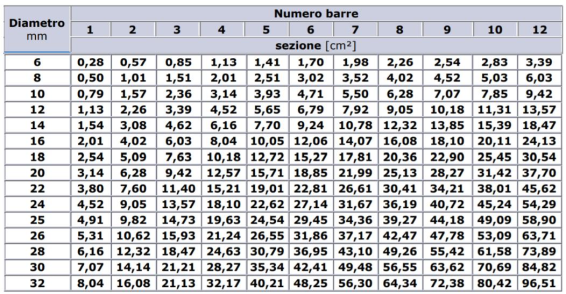
\includegraphics[width=0.7\textwidth]{immagini/dimensionamento_armatura.png} \hfill
        \caption{Valori normati delle armature da utilizzare.}
    \label{figure:pesi_muro}
\end{figure}
Si è scelto di adottare delle armature con sezione di 0.004524 \unit{m^2}, relativo a delle verghe di 24 mm di diametro, per le aree tese, ed una armatura con sezione 0.000339 \unit{m^2} per le aree compresse.

\section{Verifica agli Stati Limiti Ultimi Strutturali (SLU-STR)}
In questa sezione verrà esposto il procedimento per la verifica agli Stati Limiti Ultimi della struttura del muro; gli SLU sono le condizioni per cui la struttura dimensionata perde la finalità per cui è stata progettata, dati gli eccessivi sforzi a cui è stata sottoposta.\\
La struttura può arrivare alla condizione degli Stati Limiti Ultimi per:
\begin{itemize}
    \item crisi del calcestruzzo;
    \item crisi dell'acciaio;
    \item crisi simultanea di calcestruzzo ed acciaio.
\end{itemize}
I campi di rottura, con cui è probabile l'ottenimento di una condizione di SLU, sono sette:
\begin{itemize}
    \item campo 1-2: crisi dell'acciaio;
    \item campo 3-4: crisi dell'acciaio e/o del calcestruzzo;
    \item campo 5-6-7: crisi del calcestruzzo con acciaio in deformazione.
\end{itemize}
Per ogni tratto di muro analizzato (sezione 1, 2 e 3), si procederà ad utilizzare differenti valori del coefficiente k; in ogni caso, tale valore dev'essere compreso tra 0.259 e 0.450, relativo ai campi 3 e 4.\\
Per il campo 4 si assumono i coefficienti:
\begin{itemize}
    \item $K_b$ = 0.416;
    \item $K_{bil}$ = 0.641;
    \item $\beta$ = 0.81;
\end{itemize}
\textbf{Sezione 1 e 2-3}\\
\textbf{Coefficiente}
\begin{equation*}
    k_1 = k_2 = k_3 = f_{yd} \cdot \frac{A_s - A'_s}{\beta \cdot f_{cd} \cdot b \cdot h_1} = 391 \cdot \frac{0.004524 - 0.000339}{0.81 \cdot 17 \cdot 1 \cdot 0.46} = 0.259 
\end{equation*}
\begin{equation*}
    h_1 = h_{2-3} = s -d = 0.5 - 0.04 = 0.46 \,m
\end{equation*}
\textbf{Posizione dell'asse neutro}
\begin{equation*}
    Y_{n1} = k_1 \cdot h_1 = 0.259 \cdot 0.46 = 0.12 \,m
\end{equation*}

\subsection{Verifica SLU: momenti resistenti}
Anche per questa verifica, affinché il dimensionamento sia accettato, è necessario che la resistenza di progetto sia maggiore dell'azione di progetto. 
\textbf{Sezione 1 e 2-3}
\begin{equation*}
    \begin{split}
        M_{Rd1} = M_{Rd2} = M_{Rd3} = f_{yd} \cdot 10^{-6} \cdot A'_s \cdot (h_1-d) + \beta \cdot f_{cd} \cdot k_1 \cdot h_1 \cdot (h_1 - k_{bil} \cdot k_1 \cdot h_1) \cdot 10^6=\\
        391 \cdot 10^{-6} \cdot 0.000339 \cdot 0.46 + 0.81 \cdot 17 \cdot 1 \cdot 0.259 \cdot (0.46 - 0.641 \cdot 0.259 \cdot 0.46) \cdot 10^6 =\\
         =684177 \,Nm
    \end{split}
\end{equation*}
Le azioni di progetto calcolate sono:
\begin{itemize}
    \item Sezione 1: $M_{Ed1}$ = 47970 Nm;
    \item Sezione 2: $M_{Ed2}$ = 28067 Nm;
    \item Sezione 3: $M_{Ed3}$ = 8481 Nm;
\end{itemize}
Essendo che per tutti e tre i casi l'azione di progetto è inferiore rispetto alla resistenza di progetto, la verifica strutturale a rottura è accettata.
\subsection{Verifica SLU: resistenza al taglio}
In questo capitolo si espone la verifica alla resistenza di taglio di ogni sezione di muro, secondo le NTC-2018.\\
\textbf{Sezione 1 e 2-3}
\begin{equation*}
    kk_1 = kk_2 = kk_3 = 1 + \left(\frac{200}{h_1}\right)^{0.5} = 1 + \left(\frac{200}{0.46}\right)^{0.5} = 1.66
\end{equation*}
\begin{equation*}
    N_{Ed1} = \gamma_{G1} \cdot \gamma_{cls} \cdot H \cdot s = 1.00 \cdot 25000 \cdot 3 \cdot 0.5 = 37500 \,m
\end{equation*}
\textbf{Sforzi resisteni}\\
\textbf{Sezione 1}
\begin{equation*}
    \begin{split}
    V_{Rd1} = \left[ \frac{0.18 \cdot KK_1 \cdot \left(\left(100 \cdot \frac{f_{ck} \cdot A_{s1}}{b \cdot h_1}\right)^{1/3}\right)}{\gamma_c} +0.15 \cdot \frac{N_{Ed1}}{b \cdot k_1 \cdot h_1}\right] \cdot \left(b \cdot h_1 \cdot 10^6\right)=\\
    \left[ \frac{0.18 \cdot 1.66 \cdot \left(\left(100 \cdot \frac{30 \cdot 0.004524}{1 \cdot 0.46}\right)^{1/3}\right)}{1.5} +0.15 \cdot \frac{37500}{1 \cdot 0.259 \cdot 0.46}\right] \cdot \left(1 \cdot 0.46 \cdot 10^6\right)=\\
     = 304797 \,N
    \end{split}
\end{equation*}
\noindent
\textbf{Sezione 2 e 3}
\begin{equation*}
    \begin{split}
        V_{Rd2-3} = \left[ \frac{0.18 \cdot KK_{2-3} \cdot \left(\left(100 \cdot \frac{f_{ck} \cdot A_{s2-3}}{h_{2-3}}\right)^{1/3}\right)}{\gamma_c}\right] \cdot (b \cdot h_{2-3} \cdot 10^6) =\\
        \left[ \frac{0.18 \cdot 1.66 \cdot \left(\left(100 \cdot \frac{30 \cdot 0.004524}{0.46}\right)^{1/3}\right)}{1.5}\right] \cdot (1 \cdot 0.46 \cdot 10^6) =  283040 \,N
    \end{split}
\end{equation*}
Le azioni di progetto del muro sono:
\begin{itemize}
    \item Sezione 1: $V_{Ed1}$ = 44070 N;
    \item Sezione 2: $V_{Ed2}$ = 15565 N;
    \item Sezione 3: $V_{Ed3}$ = 41542 N;
\end{itemize}

Anche in questo caso, le resistenze di progetto risultano superiori rispetto alle azioni; pertanto, la struttura risulta verificata alla resistenza al taglio.

\section{Disegno di massima dell'opera}
Mediante il software AutoCad è stato possibile disegnare il profilo del muro e delle armature da introdurre nel momento della sua costruzione.
\begin{figure}[H]
    \centering
    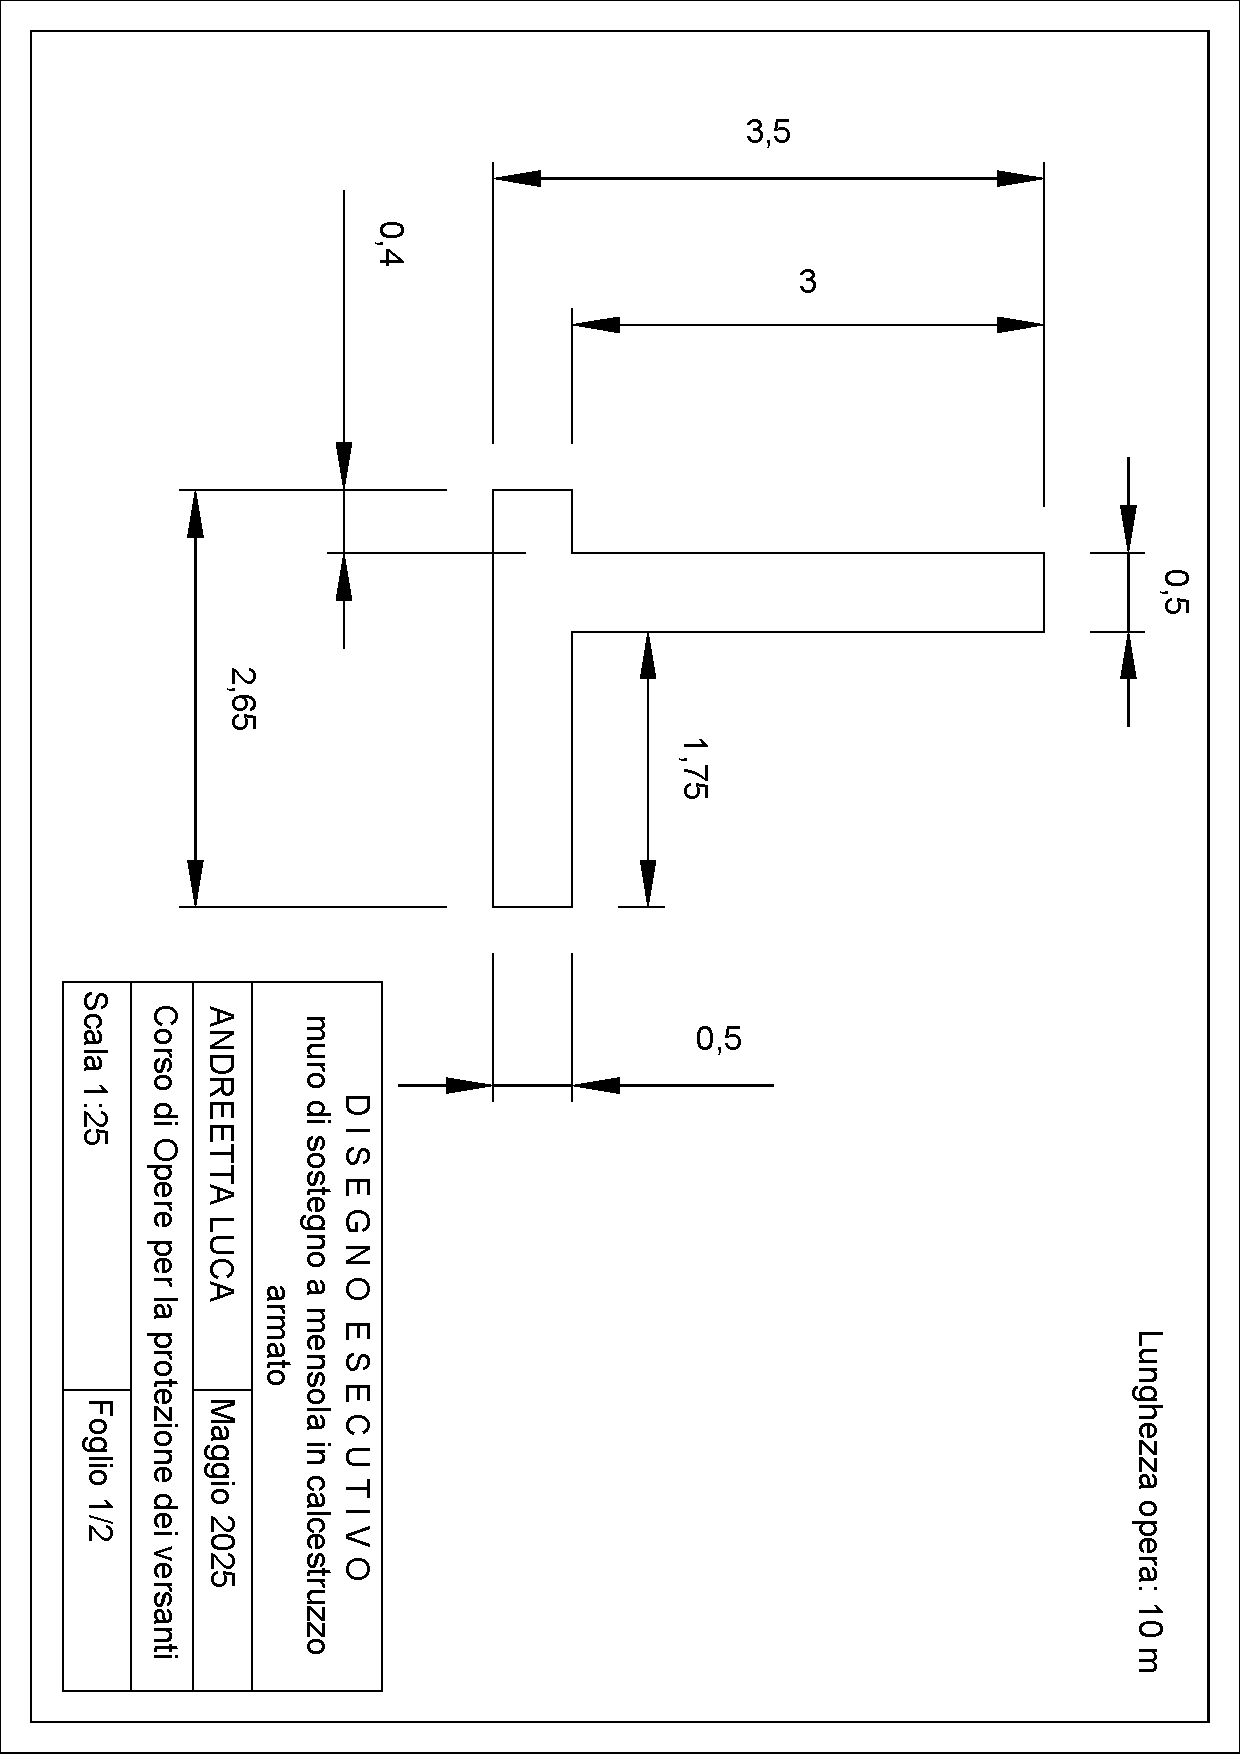
\includegraphics[width=0.5\textwidth, angle=90]{immagini/disegno_muro_cad.pdf} \hfill
        \caption{Profilo dell'opera, realizzato in AutoCad.}
    \label{figure:disegno_cad}
\end{figure}

\begin{figure}[H]
    \centering
    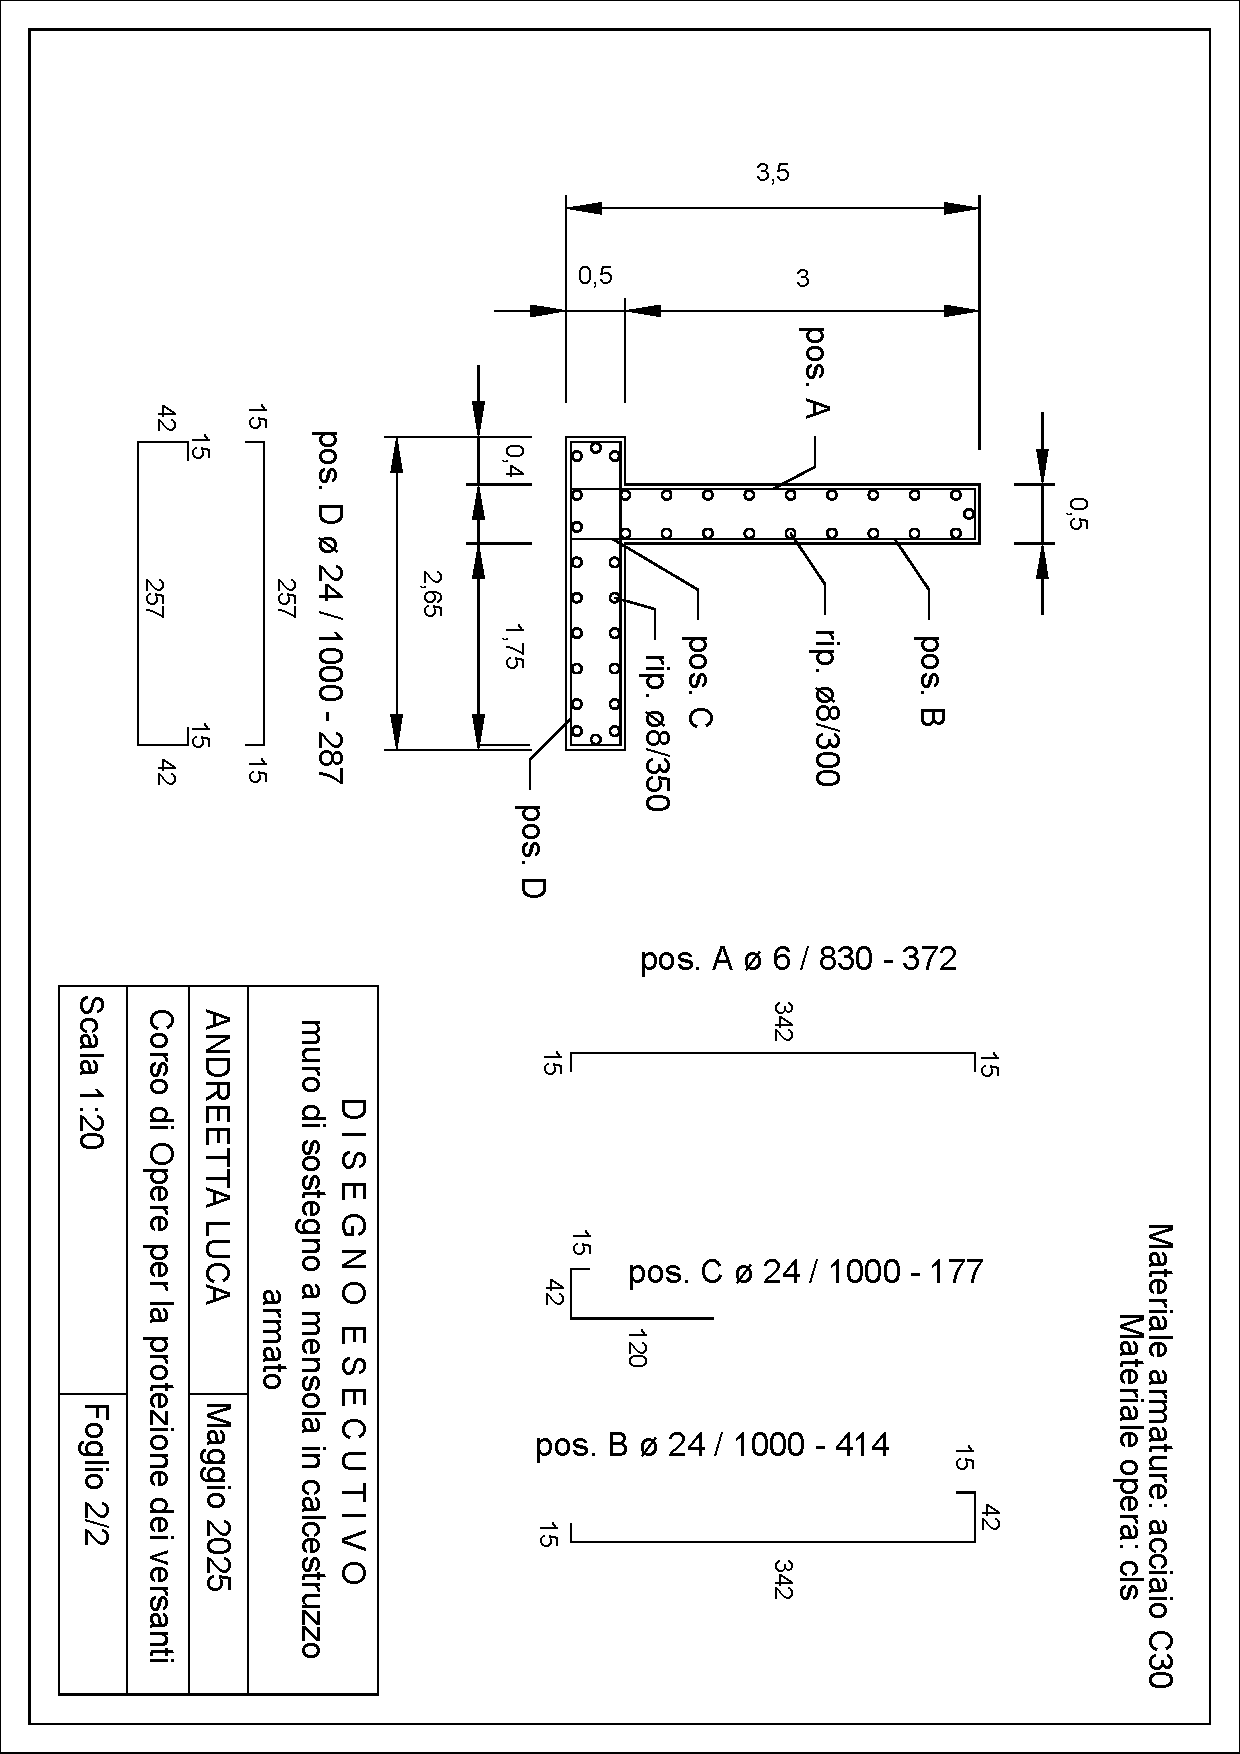
\includegraphics[width=0.7\textwidth, angle=90]{immagini/disegno_armatura_cad.pdf} \hfill
        \caption{Schematizzazione delle armature in acciaio da introdurre nel muro durante la costruzione.}
    \label{figure:stati_limit_strutturali}
\end{figure}